\chapter{Introduction}

\textit{The aim of this project was to develop a semi-supervised autoencoder-based method for classifying 
cells into phenotypes \footnote{the observable characteristics and traits of an organism} using genetic data. To this end a range 
of autoencoder based semi-supervised models have been implemented, 
ranging from fairly simple to state-of-the-art. These models were then evaluated on selected datasets, including 
the Cancer Genome Atlas expression data.}

\section{Motivation}

Classifying organisms into phenotypes using genomic data is important in both medicine and agriculture. In medicine, uses include 
classifying tissues as cancerous and non-cancerous~\cite{Li2017} and diagnosing susceptibility to Crohn's disease~\cite{doi:10.1002/humu.23280}.
In agriculture, it can be used to predict whether a crop will grow well under harsh conditions~\cite{cimmyt}.

This project used gene expression data to classify cells by specific properties of the phenotype. Gene expression is the process of synthesising 
proteins from the gene via RNA. A transcriptome is the set of all RNA 
molecules in a cell or population of cells. While every cell with a nucleus in an organism has the same DNA and genes, the cells'
gene expression differs depending on the cell type and location. This means the
transcriptome contains more than just genetic information, including information from epigenetic sources~\cite{Gibney2010}. Epigenetic differences are differences
in the phenotype without alterations to the DNA and therefore gene expression data provides more information about 
the phenotype than DNA sequencing.

Supervised machine learning techniques for classification use many pairs of data (genome) with a label
(property of phenome) to train a network, then apply that trained network to unknown data to make predictions. 
There are huge amounts of gene expression data available online, as transcriptome analysis is performed in biological labs worldwide, 
and the development of RNA-Seq using next-generation sequencing has made it even easier, but often the relevant 
label is not included. This gives researchers access to large 
amounts of data that is unusable with supervised machine learning techniques.

Semi-supervised learning attempts to leverage unlabelled data to improve the accuracy of the machine learning
algorithm on a supervised task. Autoencoders have a long history of use in semi-supervised learning problems,
being used initially to improve deep networks by pretraining them using stacked denoising autoencoders (Section~\ref{sdae})
and more recently to achieve state-of-the-art semi-supervised performance as part of the ladder 
network (Section~\ref{ladder}). This is because autoencoders are good at learning 
important features of data in an unsupervised manner, and these features are often useful in improving 
supervised performance. Semi-supervised autoencoder models should therefore allow 
allow the exploitation of data, even in absence of useful labels, in order to improve phenotype prediction.

Autoencoder-based models are implemented
using neural networks. This is advantageous because neural networks work well on non-linear data and are
also able to effectively analyse data with high dimensionality (number of features). Transcriptomes can
often contain several thousand genes, and so models must be able to cope with this level of dimensionality.

This project is also the first comparison on genomic data of the semi-supervised models described in Section~\ref{ss_models}, and is one of only a few
studies to have performed semi-supervised deep learning on genomic data.

\begin{figure}[H]
\centering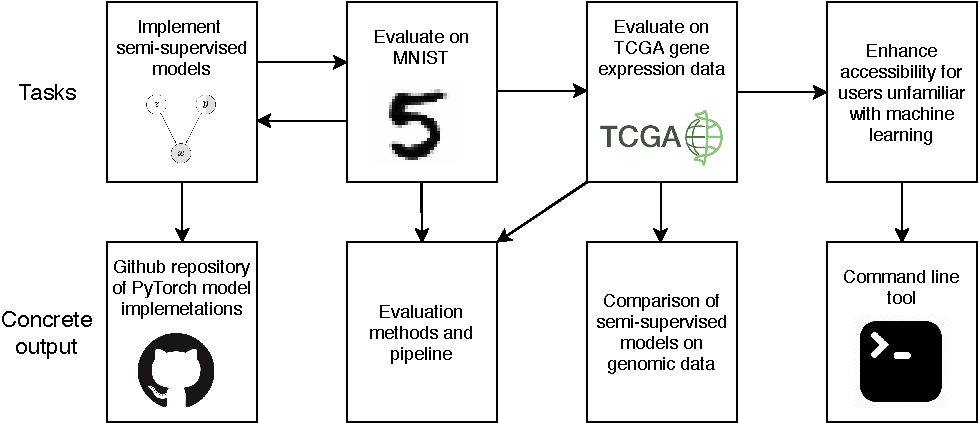
\includegraphics[scale=.9]{figs/workflow.pdf}
\caption{Project workflow}
\label{fig:workflow}
\end{figure}


\section{Related work}

Stacked denoising autoencoders have previously been used with gene expression data to derive the most informative
genes for distinguishing between healthy and cancerous cells~\cite{8217828}.

Likewise, variational autoencoders (Section~\ref{vae}) have been successfully used to extract a biologically relevant latent 
space from cancer transcriptomes ~\cite{Way2018ExtractingAB}. They and the semi-supervised variant (Section~\ref{ssVAE}) 
have also been used to model the change in the gene expression of tumours in response to certain drugs~\cite{10.1093/bioinformatics/btz158}.

Ladder networks have also been used in biologically relevant (non semi-supervised)
ways, achieving state-of-the-art accuracy in binary cancer classification~\cite{10.1007/978-3-319-78723-7_23}.